\documentclass[12pt]{article}

\usepackage[T1]{fontenc}
\usepackage[utf8]{inputenc} % L'encodage du document
\usepackage[french]{babel} % Des options supplémentaires pour que le document soit en français (noms de sections, etc.)
\usepackage{geometry}
\geometry{hscale=0.80,vscale=0.80,centering} % Permet de définir les marges (ici 10% de chaque côté)
\usepackage{amsmath}
\usepackage{amssymb}
\usepackage{amsthm} % For theorem-like environments
\usepackage{graphicx} % Ajout du package graphicx

\newcounter{definitioncounter}
\renewcommand{\thedefinitioncounter}{\arabic{definitioncounter}}

\newcommand{\definition}[1]{%
    \par\noindent\textbf{Définition \refstepcounter{definitioncounter}\thedefinitioncounter.} #1 \vspace{0.5\baselineskip}
}

\setlength{\parindent}{15pt} % Fixe l'indentation en début de paragraphe
\setlength{\parskip}{10pt} % Fixe l'espacement entre paragraphes

\begin{document}
\title{Simuler les feux de forêt}
\date{\today}
\author{Victor Sarrazin}

\maketitle

\section*{Introduction}

Avec le changement climatique, les feux de forêt sont de plus en plus fréquents et dévastateurs, à l'image de ceux en Californie en janvier 2025.

Dans ce cadre, les modélisations informatiques des feux de forêt permettent de simuler l'évolution des feux, afin de prévoir les zones à risques. Mais les simulations informatiques permettent aussi de tester l'impact de certaines transformations sur ces feux, afin de trouver des manières de réduire l'impact des catastrophes, sans pour autant dénaturer les forêts.

\section{Automates cellulaires}

Pour réaliser nos modélisations, nous allons utiliser des automates cellulaires.

\definition{Un automate cellulaire est la donnée d'un triplet $(Q, M, f)$ avec :\begin{itemize}
    \item $Q$ un ensemble d'états
    \item $M$ une matrice de taille $n \times m$, où chaque $m_{i,j}$ représente une case de la grille
    \item $f : Q^k \longrightarrow Q$ une \textit{fonction de transition} qui à l'état de la case et de $k-1$ voisins renvoie l'état suivant
\end{itemize}}

La définition de la fonction de transition dépend donc du type de voisinage utilisé. Il existe deux principaux types de voisinages, celui de \textit{von Neumann} et celui de \textit{Moore}. Nous avons choisi d'utiliser le voisinage de \textit{Moore} pour nos modélisations.

\definition{Le voisinage de \textit{Moore} est composé du noeud et de ses 8 voisins.\\ \hspace{1cm} Dans le cas du voisinage de \textit{Moore}, on a donc $f : Q^9 \longrightarrow Q$}

\pagebreak

\begin{figure}[!h]
    \centering
    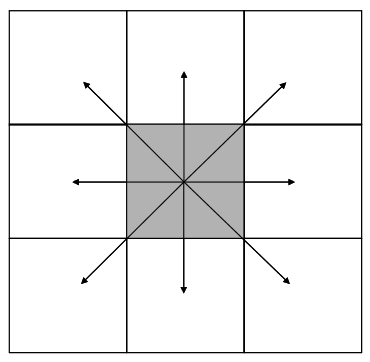
\includegraphics[width=0.20\linewidth]{pictures/moore.png}
    \caption{Voisinage de Moore}
    \label{fig:enter-label}
\end{figure}

tester

\section{Modèle d'Alexandridis}

\section{Transformations}
\end{document}